%% ----------------------------------------------------------------
%% Thesis.tex -- MAIN FILE (the one that you compile with LaTeX)
%% ---------------------------------------------------------------- 

% Set up the document
\documentclass[a4paper, 12pt, twoside]{Thesis}  % Use the "Thesis" style, based on the ECS Thesis style by Steve Gunn
\graphicspath{{Figures/}}  % Location of the graphics files (set up for graphics to be in PDF format)

% Include any extra LaTeX packages required
\usepackage[square, numbers, comma, sort&compress]{natbib}  % Use the "Natbib" style for the references in the Bibliography
\usepackage{verbatim}  % Needed for the "comment" environment to make LaTeX comments
\usepackage{missing_packages/vector}  % Allows "\bvec{}" and "\buvec{}" for "blackboard" style bold vectors in maths
\usepackage{textcomp}
\usepackage{tikz}
\usepackage{setspace} 
\hypersetup{urlcolor=black, colorlinks=true}  % Colours hyperlinks in blue, but this can be distracting if there are many links.
\usepackage{times}
\usepackage{missing_packages/lineno}
\linenumbers
\renewcommand{\figurename}{Fig.}
%% ----------------------------------------------------------------
\begin{document}
\frontmatter	  % Begin Roman style (i, ii, iii, iv...) page numbering
% Set up the Title Page
\title  {Multi Segmented Image Transfer in Delay Tolerant Networks using Bandwidth Reduction Technique}
\authors  {\texorpdfstring
            {\href{pratyush.anand@st.com
}
            {Pratyush Anand}}
            {Pratyush Anand}
            }
\addresses  {\groupname\\\deptname\\\univname}  % Do not change this here, instead these must be set in the "Thesis.cls" file, please look through it instead
\date       {\today}
\subject    {}
\keywords   {}

\maketitle

%% ----------------------------------------------------------------

\setstretch{1.5}  % It is better to have smaller font and larger line spacing than the other way round

% Define the page headers using the FancyHdr package and set up for one-sided printing
\fancyhead{}  % Clears all page headers and footers
\rhead{\thepage}  % Sets the right side header to show the page number
\lhead{}  % Clears the left side page header

\pagestyle{fancy}  % Finally, use the "fancy" page style to implement the FancyHdr headers


%% ----------------------------------------------------------------
\pagestyle{empty}  % No headers or footers for the following pages

\null\vfill
% copyright page

\cleardoublepage  % copyright page ended, start a new page
%% ----------------------------------------------------------------
%% ----------------------------------------------------------------
\frontmatter	  % Begin Roman style (i, ii, iii, iv...) page numbering

%\setstretch{1.3}  % It is better to have smaller font and larger line spacing than the other way round

% Define the page headers using the FancyHdr package and set up for one-sided printing
\fancyhead{}  % Clears all page headers and footers
\rhead{\thepage}  % Sets the right side header to show the page number
\lhead{}  % Clears the left side page header

\pagestyle{plain}  % Finally, use the "fancy" page style to implement the FancyHdr headers

%% ------------------------------------------------------------------------------------------------------
% Declaration Page required for the Thesis, your institution may give you a different text to place here
\begin{sloppypar}
\certificate{

\addtocontents{toc}{\vspace{1em}}  % Add a gap in the Contents, for aesthetics
This is to certify that the thesis titled ``Multi Segmented Image
Transfer in Delay Tolerant Networks using Bandwidth Reduction
Technique'' being submitted by PRATYUSH ANAND, Entry Number 2010EEY7515,
in partial fulfillment of the requirements for the award of the degree
of MS(R) Part Time, in Department of Electrical Engineering, Indian
Institute of Technology Delhi, is a bonafide record of the work carried
out by him under my supervision.  The matter submitted in this
dissertation has not been admitted for an award of any other degree
anywhere.
\\ \\ \\
 \\
Signed:\\
\rule[1em]{25em}{0.25pt}\\  % This prints a line for the signature
Date:\\
Prof. Subrat Kar\\
Department of Electrical Engg\\
Indian Institute Of Technology Delhi\\
New Delhi-110016 India  % This prints a line to write the date
}
\end{sloppypar}
\cleardoublepage  % Declaration ended, now start a new page
%% ------------------------------------------------------------------------------------------------------


%% ----------------------------------------------------------------
%\setstretch{1.5}  % Reset the line-spacing to 1.3 for body text (if it has changed)

% The Acknowledgements page, for thanking everyone
\acknowledgements{
\addtocontents{toc}{\vspace{1em}}  % Add a gap in the Contents, for aesthetics
I would like to express sincere gratitude to my supervisor Prof.  Subrat
Kar for giving me an opportunity to work under him. His understanding,
encouragement and guidance have provided a good basis for the thesis.  I
am deeply indebted to him for his constructive comments, fruitful
discussions and patience.

Beside my supervisor, I would express my gratitude to other members of
research committee as well for their valuable inputs and support.

I thank my colleagues at IIT delhi for their support in this journey. I
must also thank ST management for allowing me to pursue research on part
time basis.

Last but not least, I would like to thank my wife, son and parents for
their continuous support and providing me free space to complete this job.
\\
\\
\begin{flushright}
$_{\rule[1em]{10em}{0.25pt}}$\\
Pratyush Anand\\  % This prints a line for the signature
Date:\ \ \ \ \ \ \ \ \ \ \ \ \ \ \ \ \\
\end{flushright}

}


\cleardoublepage  % End of the Acknowledgements

%% ----------------------------------------------------------------



\pagestyle{plain}  %The page style headers have been "empty" all this time, now use the "fancy" headers as defined before to bring them back


%% ----------------------------------------------------------------
\lhead{\emph{Contents}}  % Set the left side page header to "Contents"
\tableofcontents  % Write out the Table of Contents

%% ----------------------------------------------------------------
\lhead{\emph{List of Figures}}  % Set the left side page header to "List if Figures"
\listoffigures  % Write out the List of Figures


%% ----------------------------------------------------------------
%\setstretch{1.5}  % Set the line spacing to 1.5, this makes the following tables easier to read
\clearpage  % Start a new page
\lhead{\emph{Glossary}}  % Set the left side page header to "Abbreviations"
\listofsymbols{ll}  % Include a list of Abbreviations (a table of two columns)
{
% \textbf{Acronym} & \textbf{W}hat (it) \textbf{S}tands \textbf{F}or \\
\textbf{DTN} & \textbf{D}elay \textbf{T}olerant \textbf{N}etwork\\
\textbf{WSN} & \textbf{W}ireless \textbf{S}ensor \textbf{N}etwork\\
\textbf{PSNR} & \textbf{P}eak \textbf{S}ignal to \textbf{N}oise \textbf{R}atio\\
\textbf{FOV} & \textbf{F}ield \textbf{O}f \textbf{V}iew\\
\textbf{SIMD} & \textbf{S}ingle \textbf{I}nstruction  \textbf{M}ultiple \textbf{D}ata\\
\textbf{PCA} & \textbf{P}rincipal \textbf{C}omponent  \textbf{A}nalysis\\
\textbf{FG} & \textbf{F}ore\textbf{g}round\\
\textbf{BG} & \textbf{B}ack\textbf{g}round\\
\textbf{BGS} & \textbf{B}ack\textbf{g}round \textbf{S}ubtraction\\
\textbf{LBP} & \textbf{L}ocal \textbf{B}inary \textbf{P}attern\\
\textbf{GMM} & \textbf{G}ausian \textbf{M}ixture \textbf{M}odel\\
\textbf{PFinder} & \textbf{P}erson \textbf{Finder} \\ 
\textbf{Vibe} & \textbf{Vi}sual \textbf{b}ackground \textbf{e}xtractor \\
\textbf{HOG} & \textbf{H}istogram of \textbf{O}riented \textbf{G}radient \\
\textbf{MIPS} & \textbf{M}icroprocessor without \textbf{I}nterlocked \textbf{P}ipeline \textbf{S}tages\\
\textbf{GCC} & \textbf{G}NU \textbf{C} \textbf{C}ompiler\\
\textbf{SOC} & \textbf{S}ystem \textbf{O}n \textbf{C}hip\\
\textbf{SD} & \textbf{S}ecured \textbf{D}igital\\
}


\setlength\parindent{20pt}

%% ----------------------------------------------------------------
\clearpage  %Start a new page

%% ----------------------------------------------------------------
\mainmatter	  % Begin normal, numeric (1,2,3...) page numbering
\pagestyle{plain}  % Return the page headers back to the "fancy" style

% Include the chapters of the thesis, as separate files
% Just uncomment the lines as you write the chapters

% Chapter 1

\chapter{Introduction} % Write in your own chapter title
\label{Chapter1}

Delay tolerant network(DTN) architecture lacks continuous end to end
connectivity. It works under some constraints like long delays and
extreme losses. For example, military network having large number of
nodes with high data mobility in extreme environmental terrestrial
conditions. Such network normally employees their own tailored routing
algorithm for high throughput based on individual's environmental
conditions~\cite{1}.\\
Now if we need to transfer image over such wireless delay tolerant
network, and that too from a live camera then it is going to become
extremely difficult task.Complexity will increases further, if we need
to build a viable low cost system with a low power battery operated
solution.  In any such cases, it would be wise to transmit
information only.We need to extract information out of image and then to
send it over the network.  Information can be of various type. So, we
need to deal that what minimum information about image allows us to
reconstruct the scenario or to detect an event. If possible then we 
need to detect event at the end DTN node itself and then to transmit
only this event information over the network.\\
Above discussed image pipeline system can also be extended to
the existing video surveillance system which are still manual. Normally
all the surveillance camera sends video to a monitoring base station,
where it is monitored by a person or a group of person. But such
arrangement can not be foolproof. So, any attempt in the direction of
its automation can be of great use in application areas such as:
\begin{enumerate}
 \item  Traffic Monitoring
  \item Elderly care
  \item Security
  \item Surveillance
  \item Assembly Line Inspection
\end{enumerate}
End goal of such an intelligent system would be to offer an
automatic analysis of scene and then to infer desired information out of
it.These systems can be lot complex because of the complexity of the
scene, specially when application is targeted for outdoor monitoring.
Sometime background of the scene can be moving, while in some
other scene ambient light can be different. Detection of foreground
objects becomes a trivial task in whole of this pipeline.Once we have
foreground objects, we can save a lot of bandwidth if we can detect if
object is of our interest or not.\\
In the current work, we are targeting to detect moving person and
then to send it's information such as location, time of detection etc to
the monitoring station. We want to keep our pipeline computation cost
very low, at the same time with high genuine detection rate and low
false detection rate.


\section{Past Work and Literature Survey}

\subsection{Image transfer over DTN/Low BW networks}

There has been no data available for the image transfer over terrestrial
DTNs, however there has been several attempts ~\cite{2, 3, 4, 5} to transfer
image over low bandwidth wireless sensor networks (WSN).

Georgiy et al. ~\cite{2} have tried to transfer different versions of JEPG
images over zigbee network and then has done performance comparison.
This works shows that there is an effect of compression coding algorithm
on peak signal to noise ratio(PSNR). It has been observed that
compression technique with scalable coding is more error tolerant in WSN
environment.Hengstler et al. ~\cite{3, 5} have gone step ahead and have used 3
cameras. One high resolution camera and two low resolution cameras. Low
resolution cameras are used for stereo matching and to identify any
moving object in the camera's field of view (FOV). If a moving object is
found then only high resolution camera is triggered. Such system is
power efficient in  comparison to the camera mote continuously
transmitting JPEG frames. Chen et al. ~\cite{4} have used xetal parallel
processors for image processing. After subtracting background, ellipse
fitting has been done on the foreground object. This elliptical
information is collected from different camera and 3D view is
reconstructed from it. 

\begin{figure}[!b]
\centering
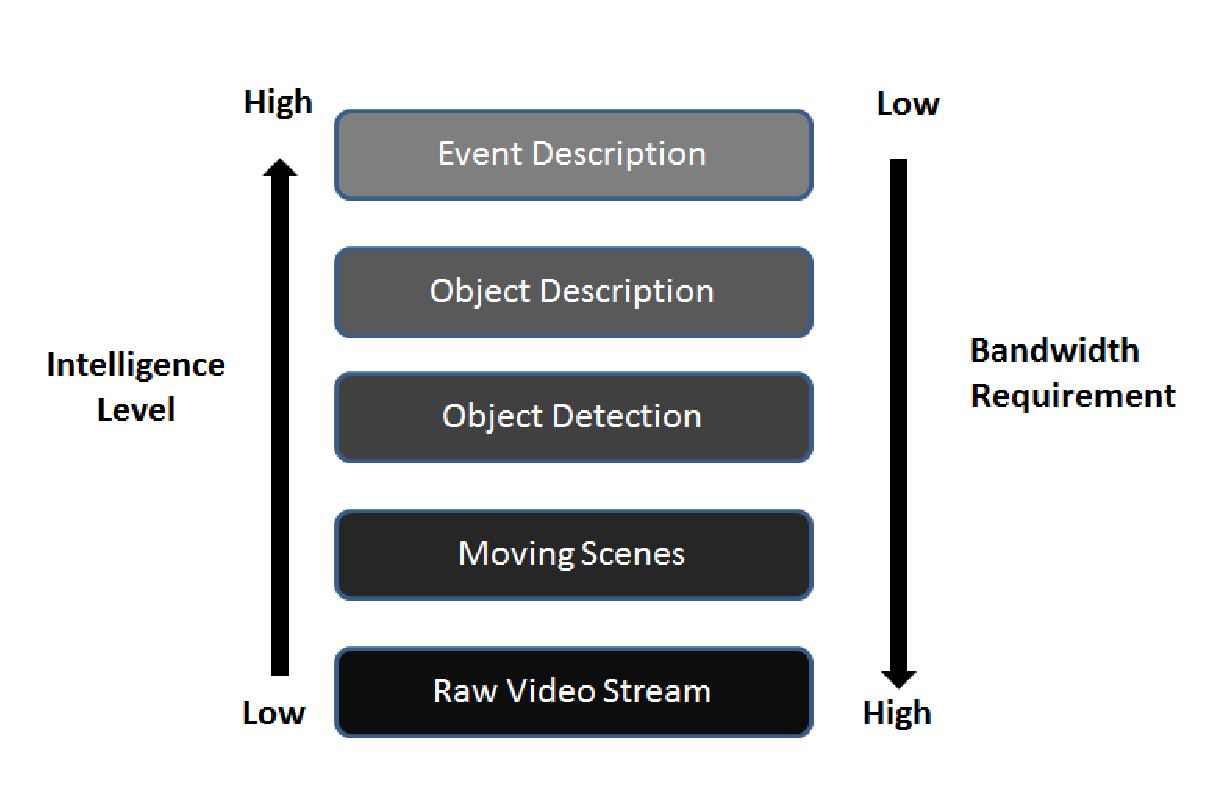
\includegraphics[scale=0.80]{Figures/image_tr_level}
\caption{Surveillance image transfer level, reproduced from ~\cite{3}}
\label{image_tr_level}
\end{figure}

Figure ~\ref{image_tr_level} shows different level of intelligence at
which data can be transmitted in an augmented video surveillance
system. As we go above in the hierarchy, we attain higher level of
intelligence and save lot of bandwidth. But all these come at the cost
of computational power of mote node.

\subsection{Image size reduction techniques}
Most of the image intensity information are not distinguishable by human
eye, so they are irrelevant. Normally, neighbouring pixel of an image
are co-related to each other, so they are redundant. Such redundancy is
called spatial redundancy.Coming to the video, they are composed of
large number of still images , which have been taken at very short
interval of time. So, it is expected that there would be lot of temporal
redundancy between two neighbouring frames.  Therefore an image
compression technique is developed around basic principal of reducing
irrelevancy and redundancy. Broadly, compression techniques are
categorised in lossless and lossy ~\cite{6}. In a lossless compression, original
image can be retrieved exactly, but it does not gives much compression.
Reconstructed image after a lossy compression degrades in quality,
however they provide good amount of compression. We do not need to
reconstruct exact image for surveillance applications. So maximum
possible compression would help a lot of bandwidth on network.\\

Most of the video coding method are based on transform coding followed
by predictive coding based on motion estimation. Such methods are called
block based method, where prediction is implemented on a complete block.
MPEG-1,2 come in this category. However,algorithm based on object based
coding techniques ~\cite{7, 8} including MPEG-4 provides substantially
better compression. Chaudhury et al. ~\cite{7} have used principal
component analysis (PCA) method for object segmentation.Further, they
have reused tracking subspace for object coding which substantially
reduced computational time. Babu et al. ~\cite{8} have calculated motion
between current and previous frame. Further motion compensated error and
other object parameters such as boundary, location and motion
information has been coded using suitable source coding techniques.  

\subsection{Background subtraction techniques}
In any object based method, focus is on foreground object (FG) which is part
of actual information.The most simple way of getting FG objects is to
find difference with the previous frame. Offcourse it is computationally
least expensive , but does not work for most of the practical
cases. Basic of all background (BG) modeling algorithm is to find an
image pattern which does not have any moving object. However, this is a
very complex task, as sometimes camera itself might be moving, in some
other cases lighting condition can vary a lot.In some cases even all the
moving objects might not be of interest. For example, escalator is the
part of BG in a scene where a person is standing on a moving
escalator.\\
Many methods ~\cite{9, 10, 11, 12, 13, 14} have been developed for the background
subtraction (BGS), having strength and weakness in terms of computation
complexities and performance. Frame differencing is of lowest
computational complexity. Here simply current frame is subtracted with
the last frame, and if absolute of the subtracted value is less than a
threshold value, then that pixel is made part of BG. Biggest drawback of
this method is that if an FG object stays for more than a frame time at
any position then that is made part of BG. Further, if an FG object is
consist of almost uniformly distributed intensities, then internal
portion of the object is considers as BG. However, there is one biggest
advantage of this method is that, it is quickly adaptable to the change
in scene, as it depends on only last frame.\\
BGS algorithm ~\cite{10, 12, 13, 14} based on Gaussian average or median of
last couple of frames, comes in the category of middle level of
computational cost. Wren et al. ~\cite{12} have used running average of
last n frames as BG model. Algorithms based on median filter show better
performance, but it has more memory requirement compared to running
average. Here, median of last n pixel is considers as BG model.
McFarlane et al. ~\cite{14} have used modified version as average median
filter, which has memory requirement same as that of frame differencing.
Here, if a pixel value is greater than the corresponding BG pixel, then
BG pixel value is incremented by 1, and if it is less then decremented
by 1.\\
Yao et al. ~\cite{11} have used a method based on local texture features
represented by local binary patterns (LBP) and photometric invariant
color measurements in RGB color space. Texture is an important
characteristic of images and video. LBP is invariant to any monotonic
gray level change. Also, it is computationally very simple. LBP operator
labels image pixel of a cell by thresholding the neighborhood of each pixel
with the center value and considering the result as a binary number.

LBP binary code of a pixel is calculated as follows:
\begin{equation}
LBP_{NR} = \Sigma _{n = 0} ^{N - 1} f(I_c - I_n) 2^n \hspace{20 mm} where f(x) = \left\{ 
  \begin{array}{l l}
     1 & \quad \text{if $x$ $\geq$  $0$}\\
     0 & \quad \text{otherwise}
   \end{array} \right.
\end{equation}
Here, $I_c$ is the gray value of central pixel and I$_n$ are the gray
value of pixels at a distance of radius R.  On a multi channel color
image LBP can be calculated at each pixel separately.LBP works well with
local illumination changes, however there can be issues in case of
global illumination change.LBP fails when both background and foreground
of an image shares same texture information. Yao et al. have used
photometric invariant color features in RGB color space to overcome this
limitation of LBP.

\subsection{Object detection techniques}

\subsection{Outstanding issues}

\section{Motivation}
what and why I will do?

\section{Organisation of thesis}
 % Introduction

% Chapter 2

\chapter{Methodology and approach} % Write in your own chapter title
\label{Chapter2}

\section{Image analysis tools}
\indent Matlab and OpenCV~\cite{34} are two highly used image
processing tools.  Matlab comes with rich image processing and analysis
libraries. It supports most of the work discussed in introduction
chapter. Matlab also provides interface to convert the code into a C
code. However, generated C code is normally very bulky and takes higher
execution time. OpenCV is an open source computer vision library
initiated by Intel. It is available at
http://SourceForge.net/projects/opencvlibrary. It can be used for
research or even commercial purposes. Unlike GNU Public License (GPL),
it's licensing does not force that modifications to the library be made
public. \\
\indent OpenCV has been mainly developed in C and C++ on Linux platform.
However, interfaces for other scripting / programming language such as
Python, Ruby, Java etc have also been developed. Libraries are also
available for windows, Android and Mac OS platform. OpenCV libraries
have been used in many applications since its first release in 1999.
Range of applications varies from stitching street view images together,
detecting intrusions in surveillance video, monitoring mine equipment,
helping robots navigate and pick up objects, detection of swimming pool
drowning accidents, running interactive art, checking runways for
debris, inspecting labels on products in factories, to rapid face
detection.\\
\indent OpenCV design goal is to build computer vision library with
computational efficiency which can work with real time applications. It
contains functions in almost all the area of image processing  and
computer vision like, histogram processing, morphological processing,
segmentation, detection tracking, camera calibration etc. Therefore,
selection of OpenCV libraries allows faster evaluation and development
of real embedded application.\\
\indent OpenCV libraries are also available for embedded architecture
CPUs like ARM. This allows easy porting of applications developed on x86
platform to ARM or other embedded platforms.\\
\indent Therefore, we decided to implement our image processing
algorithms in C and on Linux platform, so that it can easily be ported
from a PC to embedded environment. Wherever possible, we have used
OpenCV library.
\section{Surveillance image processing flow}
\indent Top level surveillance image processing flow for a low bandwidth
network is as shown in Fig.~\ref{image_pipeline}. End goal of low
bandwidth implementation would be to generate information such as human
detected, their position and the time of detection. So, for above
implementation we have to decide on following items, computational
efficiency and true detection for considered object has to be kept as
primary objective while making any decision.

\begin{figure}[!b]
\centering
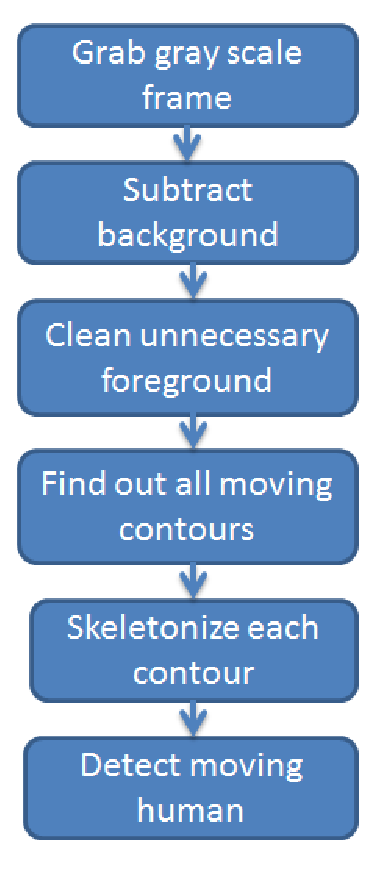
\includegraphics[height=100pt]{Figures/image_pipeline}
\caption{Low BW surveillance image application flow}
\label{image_pipeline}
\end{figure}
\begin{enumerate}
\item \textbf{Background Subtraction:} Methods based on LBP by Yao et
	al.~\cite{11} have striking nice result. It works superbly with
	varied background situation like wavering tree, moving escalator
	etc. Barnich et al.~\cite{9} claim that Vibe which uses random
	sample selection also performs well in all situation and have
	extremely low computational cost. Yao et al. have provided their
	C code, however Barnich et al.  have only provided an object
	library for x86 platform. Therefore we need to first code vibe
	in C and then to compare above two algorithms.
\item \textbf{Detection and Tracking:} Method based on skeleton motion
	features~\cite{32, 22, 31} seems to be computationally
	efficient. So we need to evaluate different method of
	skeletonization, suitable for motion calculation. Performance of
	detector based on such method need to be compared with other
	methods based on covariance feature with cascade of logitboost
	classifier~\cite{19}  and Haar-like like features~\cite{17} for
	which C codes are already available in public domain.
\item \textbf{Embedded implementation:} It is very important to see
	performance of pipeline based on different algorithm on real
	embedded platform. ARM controller is used in most of the
	embedded multimedia applications. So, it will be nice to observe
	their performance with ARM controller.
\end{enumerate}
\section {Evaluation of different techniques for pipeline stages}
\subsection{Frame acquisition}
\indent OpenCV provides a way to grab frames either from a camera or
from a file. cvCaptureFromFile or cvCaptureFromCAM returns CvCapture *
struct which can further be used to query frame from either a test video
file or from camera respectively. cvQueryFrame function reads one frame
and returns its pointer. If camera's output or test video is in RGB mode
then, it need to be converted into gray scale image for further
processing. cvCvtColor function has been used to convert image from RGB
to gray scale.
\subsection{Background removal}
\indent Since background subtraction has key role in accomplishing
intended job, therefore we have compared two recently developed~\cite{3,
5} efficient background subtraction algorithm and then selected one of
them~\cite{5} in our final work.  The method described by Yao and
Odobez~\cite{3} is based on use of texture features present in Local
Binary Pattern (LBP).  LBP works well with local illumination changes,
however there can be issues in case of global illumination change. They
have carried out several improvements by using photometric invariant
color measurement and flexible weight updating for background
modes.However, our experiments says that, computationally it is very
less efficient compared to method proposed by Barnich et al.~\cite{9},
which is based on unique way of replacing background pixel value over
the time. It replaces background values for last N frames randomly.
Furthermore, it diffuses updated values to neighbouring pixels, and
again that too on random basis. We have selected method by Barnich et
al.~\cite{9} in our final pipeline, because of its computational
efficiency while maintaining quality.  Fig.~\ref{bg_compare} shows the
comparison of execution time of these two algorithm.

\begin{figure}[!t]
\centering
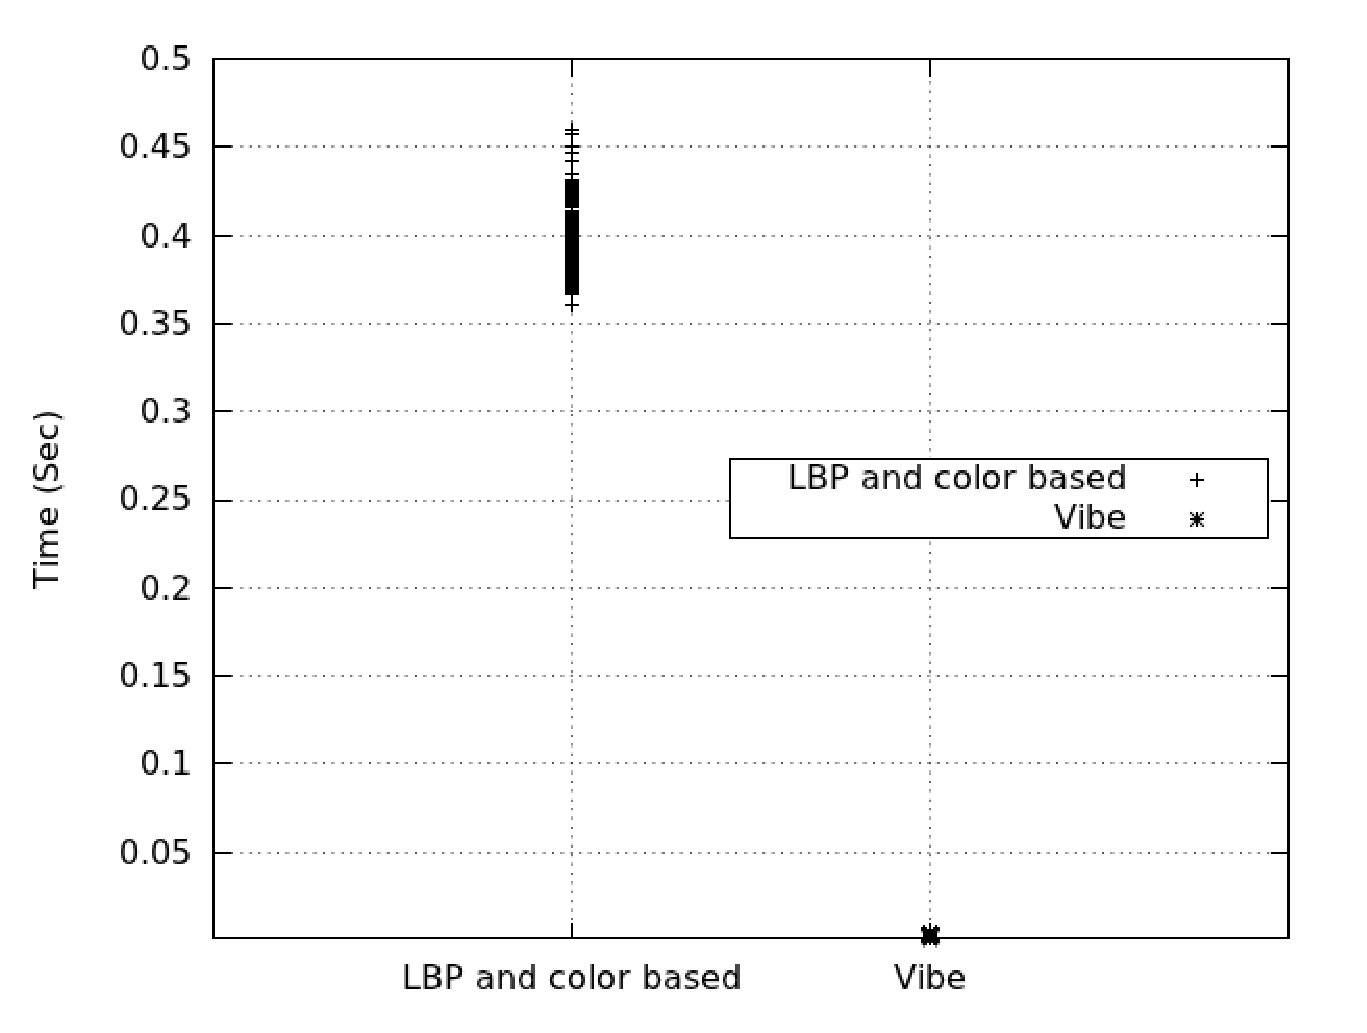
\includegraphics[height=300pt]{Figures/bg_compare}
\caption{Variation of background subtraction execution time of~\cite{11}
and~\cite{9} with frame number. This timing was observed with a system
having having DMIPS = 800.}
\label{bg_compare}
\end{figure}
\subsection{Noise removal}
\indent None of the background subtraction algorithm allows pure
foreground extraction. There would always be several noise objects in the
extracted image. These are cleaned by morphological erosion operation
(cvErode) followed by dilation (cvDilate) operation. Further all moving
contours are separated out by using OpenCV library function
cvFindContours. This function provides us boundary point of individual
moving object.
\subsection{Skeletonization techniques}
\indent Image skeletons are nice way to represent shape of an object.
This method can be used to identify type of object. We have evaluated
different skeletonization techniques, with their merits and demerits for
suitability to our requirement.
\begin{enumerate}
\item \textbf{Contour skeleton:} It is obtained by finding outer
	boundary points of an object. It gives idea about global shape
	of an object. Boundary points obtained by function
	cvFindContours can further be converted into polygon by
	cvApproxPoly. Vertices of this polygon connected together gives
	an idea about outer shape of the object. An example of such
	skeleton has been shown in Fig.~\ref{skeletons}.A.

\begin{figure}[!t]
\centering
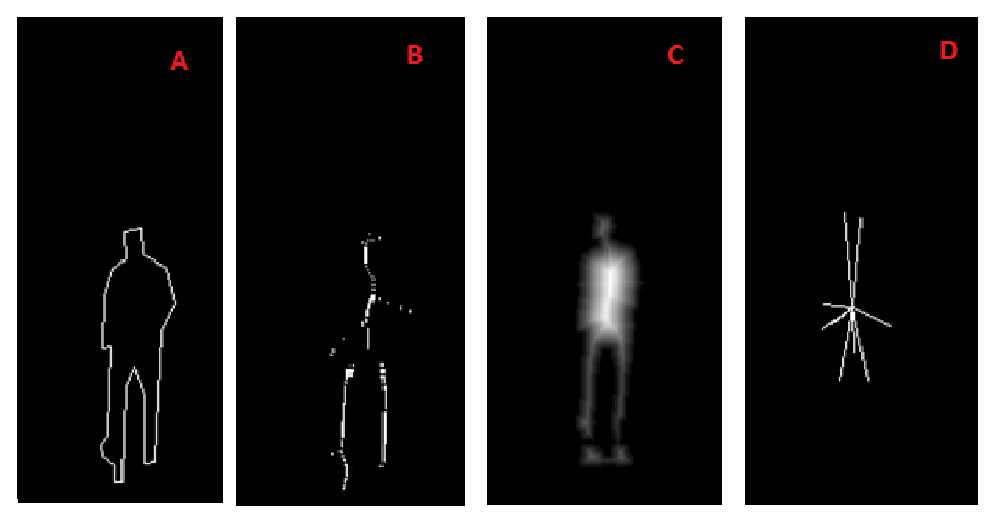
\includegraphics[height=220pt]{Figures/skeletons}
\caption{Skeleton obtained by different methods. \textbf{A.} Contour
skeleton \textbf{B.} Morphological skeleton \textbf{C.} Distance
transform skeleton \textbf{D.} Star skeleton}
\label{skeletons}
\end{figure}
\item \textbf{Morphological skeleton:} Gonzalez and Woods have provided
	a set of morphological operations in their book Digital image
	processing~\cite{35}, which has defined morphological
	skeletonization as follows:
	\begin{equation}
	\begin{aligned}
		S(A) &= \Sigma ^K _{k = 0} S_k(A) \label{morph_skel}\\
	\mathrm{where} \hspace{5 mm} S_k(A) &= (A \ominus kB) - (A \ominus kB) \circ B \\
			  k &= max \{ K | (A \ominus kB) \neq \phi\}
	\end{aligned}
	\end{equation}
Translating Eqn~\ref{morph_skel} into C code:
\begin{lstlisting}

	do
	{
		cvErode(img, eroded, element, 1);
		cvDilate(eroded, temp, element, 1);
		cvSub(img, temp, temp, NULL);
		cvOr(skel, temp, skel, NULL);
		cvCopy(eroded, img);
		done = (cvCountNonZero(img) == 0);
	} while (!done);

\end{lstlisting}
\indent An example of skeleton obtained by morphological method has been
shown in Fig.~\ref{skeletons}.B.
\item \textbf{Skeleton by distance transform:} Distance transform of an
	input image is obtained by creating a new image where pixels are
	set to a value equal to the distance to the nearest zero value
	pixel in input image. We have seen that the contour skeleton
	provided outer shape of the object, where as distance transform
	method provides internal orientation of object. OpenCV provides
	a function cvDistTransform, which can be used to build a
	distance transformed image. An example of skeleton obtained by
	distance transform method has been shown in
	Fig.~\ref{skeletons}.C.
\item \textbf{Star Skeleton:} In this method we plot distance of each
	boundary point from the centroid and then use peaks of the curve
	as skeleton point.
\begin{enumerate}
\item Centroid of each object is found out using following
	Eqn~\ref{centroid_calc}.
	\begin{eqnarray}
	C_x = {1 \over N} \Sigma ^N _{i = 1} X_i \label{centroid_calc}
\nonumber \\
	C_y = {1 \over N} \Sigma ^N _{i = 1} Y_i 
	\end{eqnarray}
Here X$_i$ and Y$_i$ are (X,Y) co-ordinates of i$_{th}$ point on the contour
boundary.
\item Distance d$_i$ is calculated between centroid and each boundary
	point as follows.This calculated distance vector are stored in a
	CvMat array.
	\begin{equation}
	d_i = \sqrt{(C_x - X_i)^2 + (C_y - Y_i)^2} \label{dist_calc}
	\end{equation}

\begin{figure}[!t]
\centering
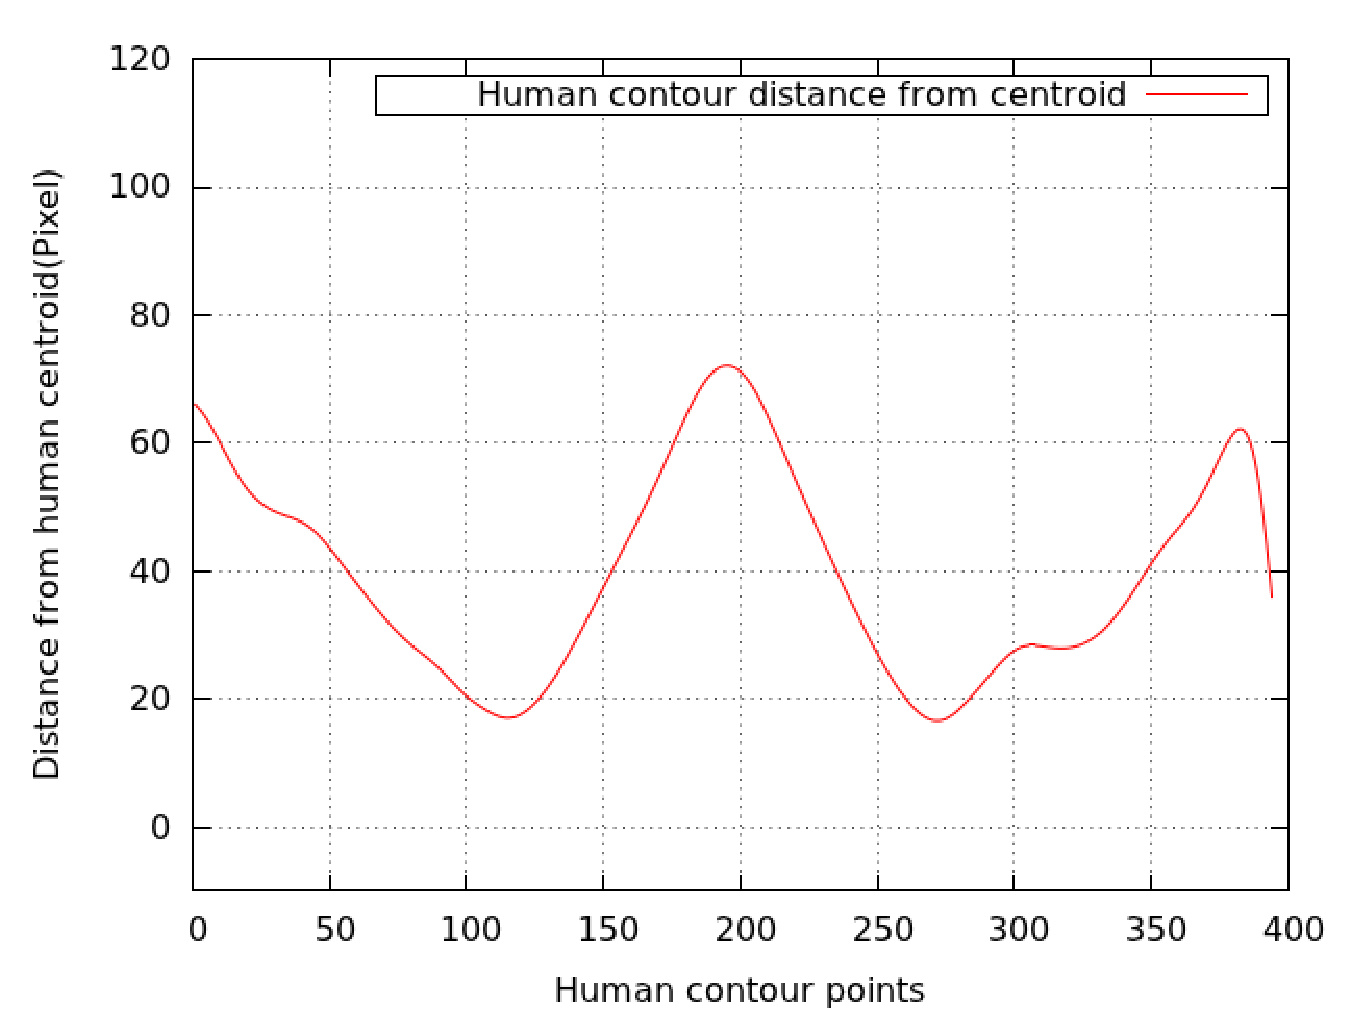
\includegraphics[height=200pt]{Figures/distance}
\caption{Distance plot of human contour points from its centroid}
\label{distance}
\end{figure}
\item Distance vector array is smoothed to remove noise peaks using
	cvSmooth. If these distances are plotted then it looks like
	Fig.~\ref{distance}. Now local maxima of distance vector is
	calculated by finding zero crossing of difference vectors. These
	local maxima provides a star form of skeleton centered at
	centroid of the object. A typical star skeleton has been shown
	in Fig.~\ref{skeletons}.C.
\end{enumerate}
\end{enumerate}
\subsection{Human detection methods}
\indent We have evaluated three methods of human detection technique mainly on the
basis of their computation efficiency.
\begin{enumerate}
\item \textbf{Detection using covariance features:} We have used method
	implemented by Yao et al. ~\cite{19}. We have selected this
	method, because it has been widely referenced and also the
	source(C code) is available in public domain.\\
\item \textbf{Detection using Haar-like features:} We have evaluated
	work by Viola et al.~\cite{16, 17} which uses Haar-like like
	features for human detection. Again, reason to evaluate this
	algorithm was same, that it has been widely discussed and
	referenced.
\item \textbf{Detection using skeleton motion features:} We have
	evaluated this method as it seems to be computationally very
	efficient.  We have done our own implementation in C to evaluate
	this method.  Human motion can be represented suitably by
	movement of legs. So, we use star skeletonization method which
	seems best suitable for human leg motion analysis. We have seen
	that star skeletonization gives us skeleton points in form of peak
	distance from centroid. However, some of these peak points are
	not of our interest. In our algorithm, we are using 2 most relevant
	peaks which are nearest to each bottom corner of bounding box of
	contour respectively. Only these two peaks along with centroid
	will give us sufficient information to distinguish human among
	human, vehicle or animal etc.\\
\indent For human subjects, the two peaks correspond to the two legs of
human. For vehicles, the peaks correspond to the two extrema points of
lower portion of back and front.  When it is an animal, the peaks
correspond to front and back leg of animal.\\
\item Let P$_1$(X$_1$, Y$_1$), P$_2$(X$_2$, Y$_2$) and C(C$_x$, C$_y$)
are two peaks nearest to bottom right and bottom left corner and
centroid respectively. Let $\theta$ is the angle between the line
segments P$_1$C and P$_2$C, then $\theta$ can be calculated as
follows.\\
%
	\begin{equation}
	\theta = tan^{-1}[(Y_2 - C_y) / (X_2 - C_x)] \\ - tan^{-1}[(Y_1 - C_y) / (X_1 - C_x)]
	\end{equation}
%
\indent If variation of $\theta$ is plotted in respective frames for
human and vehicle then the resultant plot is as shown in
Fig.\ref{angle_plot}.  The observations from this plot is that for a
human subject, angle variation pattern is repeatable, and it is zero for
almost at regular intervals.  For vehicle, it is constant. The
experiment with images containing animal is yet to be done. For images
with animals in it, there are variations with repeatable patterns but
which never touch zero.  These criterion can be the basis to identify an
object, and to decide whether it is a human,vehicle or animal.

\begin{figure}[!t]
\centering
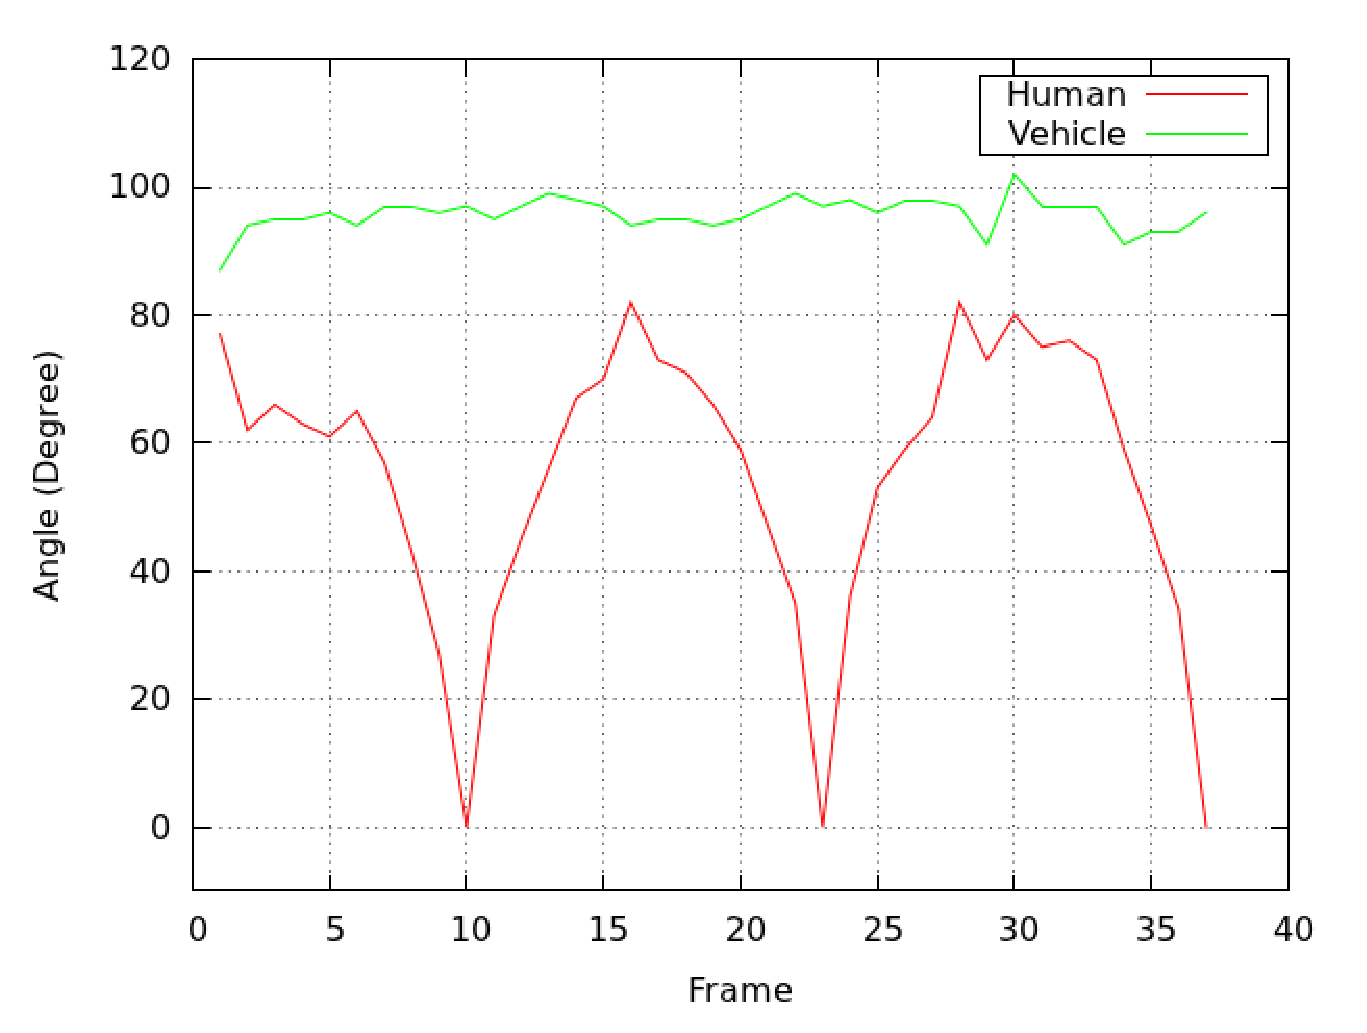
\includegraphics[height=300pt]{Figures/angle_plot}
\caption{Plot of variation of angle $\theta$ with frame number for human and
vehicle.}
\label{angle_plot}
\end{figure}
\item Every new object which comes into the field of view is tracked and
	value of (C$_x$, C$_y$), $\theta$ in each frame is stored. 
\begin{enumerate} 
\item We track value of $\theta$ until it goes to zero three times.
\item Now we consider $\theta$ values between first and second zero as
vector T$_1$ and $\theta$ values between second and third zero as vector
T$_2$.
\item We find mean m$_1$ and m$_2$ of vector T$_1$ and T$_2$ respectively.
\item If n is the length of vector T$_1$ then, we calculate correlation
value (r) between these two vectors to find similarities as follows.
	\begin{equation}
	r = {{\Sigma ^n _{i = 1}(T_{1i} - m_1) . (T_{2i} - m_2)}
\over {\sqrt {\Sigma ^n _{i = 1} (T_{1i} - m_1)^2 . \Sigma ^n _{i = 1} (T_{2i}
- m_2)^2}}}
	\end{equation}
\item If correlation value is greater than a threshold value TH$_1$,
then we conclude that it is a human.
\end{enumerate} 
\end{enumerate} 
 %methodology and approach

% Chapter 3

\chapter{Embedded Implementation} % Write in your own chapter title
\label{Chapter3}
We have done evaluation of embedded solution of our implementation on
the basis of following:
\begin{itemize}
	\item \textbf{Low cost:} It is very important for any mass
		market product.
	\item \textbf{Low power:} Reducing energy consumption is a
		movement and is necessary for a greener world.
		Technically also it is very important for a prolonged
		battery life.
	\item \textbf{Rapid software development:} Today lot of software
		is available in every domain of science by open source
		community. Platform must be developed by considering
		re-usability of available software in public domain.
\end{itemize}
\section {Hardware Evaluation}
discuss different embedded architecture and justify why ARM is best
choice. Memory and other component requirements etc.
\section {Software Evaluation}
discuss about different options like bare code without any OS, other
open source OS and finally Linux. Justify uses of Linux.
\section {Component of embedded Linux software}
\subsection {Toolchain}
cross toolchain, why and how
\subsection {BootROM}
why and how, if not then other alternatives.
\subsection {First level boot loader}
ddr initialization code, why and how
\subsection {Second level boot loader}
preparation of OS booting, why and how
\subsection {Second level boot }
preparation of OS booting, why and how
\subsection {Operation System}
preparation of Linux booting. Minimal Linux component needed
(menuconfig) for our implementation. Also discuss about V4L2 camera
framework.
\subsection {Root filesystem}
RFS, what, why and how
 %results and conclusion

% Chapter 4
\chapter{Results and conclusion} % Write in your own chapter title
\label{Chapter4}
\indent We have discussed different background subtraction and human
detection techniques in chapter ~\ref{Chapter2}. We have also discussed
about SKELMOT, technique used for human detection in our work. In this
section we discuss results of different evaluations and also how does
SKELMOT compares with others. We also draw conclusions from our results
and future works to be done.
\section{Results}
\indent We did comparison of execution time of background subtraction
algorithm in Fig.~\ref{bg_compare}. Graph shows that Vibe is far more
computationally efficient compared to other. Therefore we used Vibe
algorithm in SKELMOT, where we target human detection based on its
skeleton motion.\\
We have seen different skeleton
output in Fig.~\ref{skeletons}. We have also seen that star skeleton
provides a simple way for leg motion analysis. Therefore we have used
Vibe~\cite{9} as background subtracter and \textbf{Skel}etonized
\textbf{M}otion \textbf{A}nalysis (SKELMOT) based on star skeleton for
object detection in our final implementation.\\
\indent We conclude that with our implementation, system is able to
detect a moving person after it's 3 steps move.
Fig.~\ref{pipeline_images} shows output images at different stages of
pipeline.
\indent We have also done experiments with negative images like a person
moving on bicycle, or a vehicle moving on road. SKELMOT is successfully able
to discriminate between these objects. Fig.\ref{negative_inputs} shows
how it rejects moving vehicle and bicycle and  does not detect them as
human.

\begin{figure}[!t]
\centering
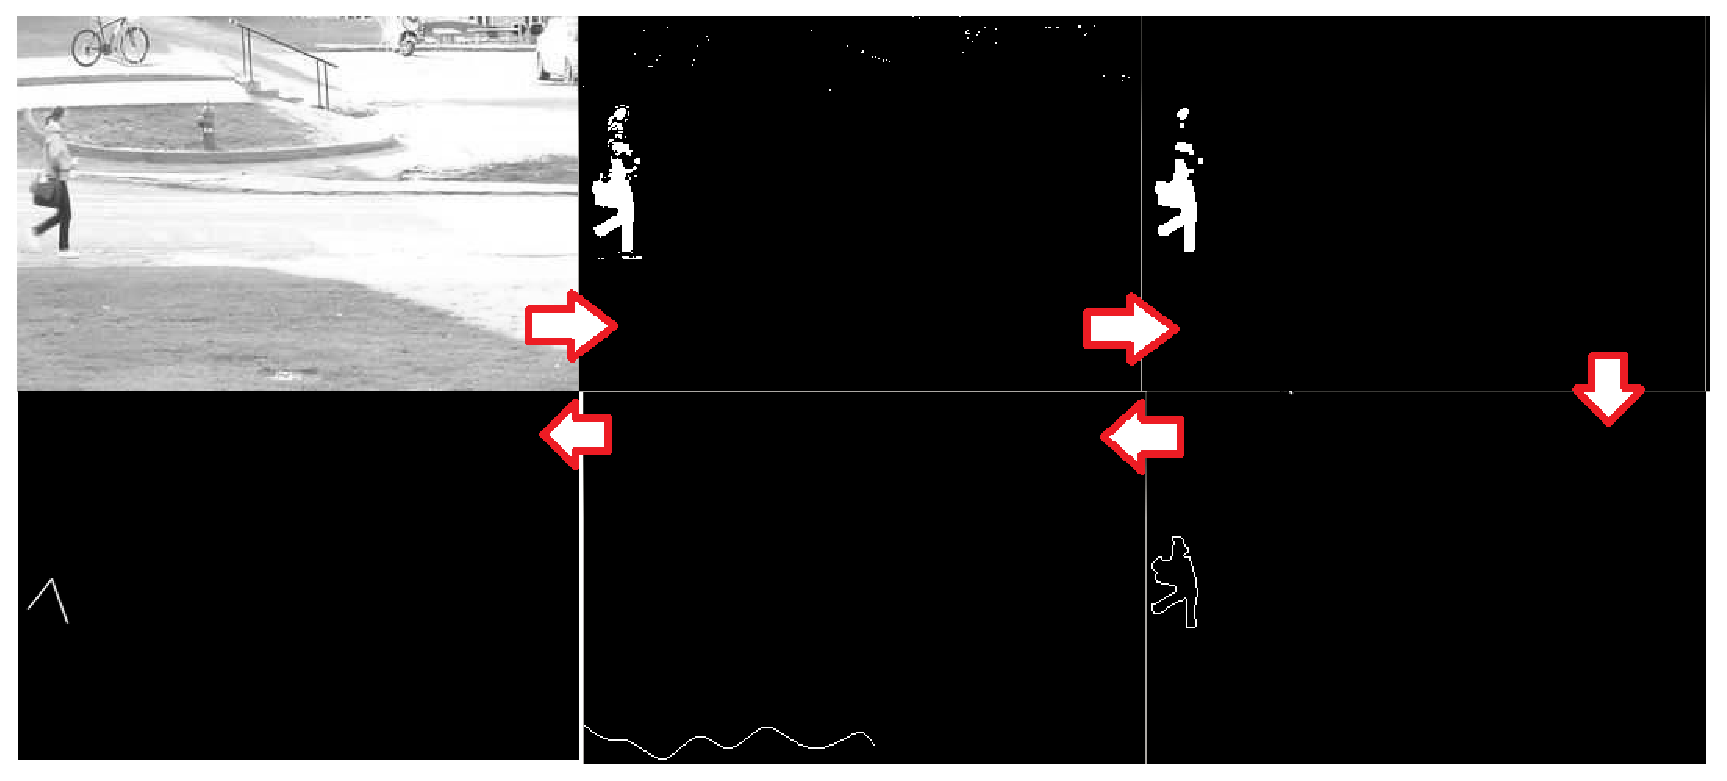
\includegraphics[height=200pt]{Figures/pipeline_images}
\caption{Images at different stages of implementation. (From top left in
clockwise order) \textbf{a.} Gray Scale input frame
\textbf{b.}Foreground extracted image using Vibe \textbf{c.} Cleaned
image \textbf{d.} Contour of moving object \textbf{e.} Plot of 3 points
of interest, centroid and two distance peaks nearer to bottom left and
bottom right corner of bounding box \textbf{f.} Virtual representation
of scene} 
\label{pipeline_images}
\end{figure}
\begin{figure}[!b]
\centering
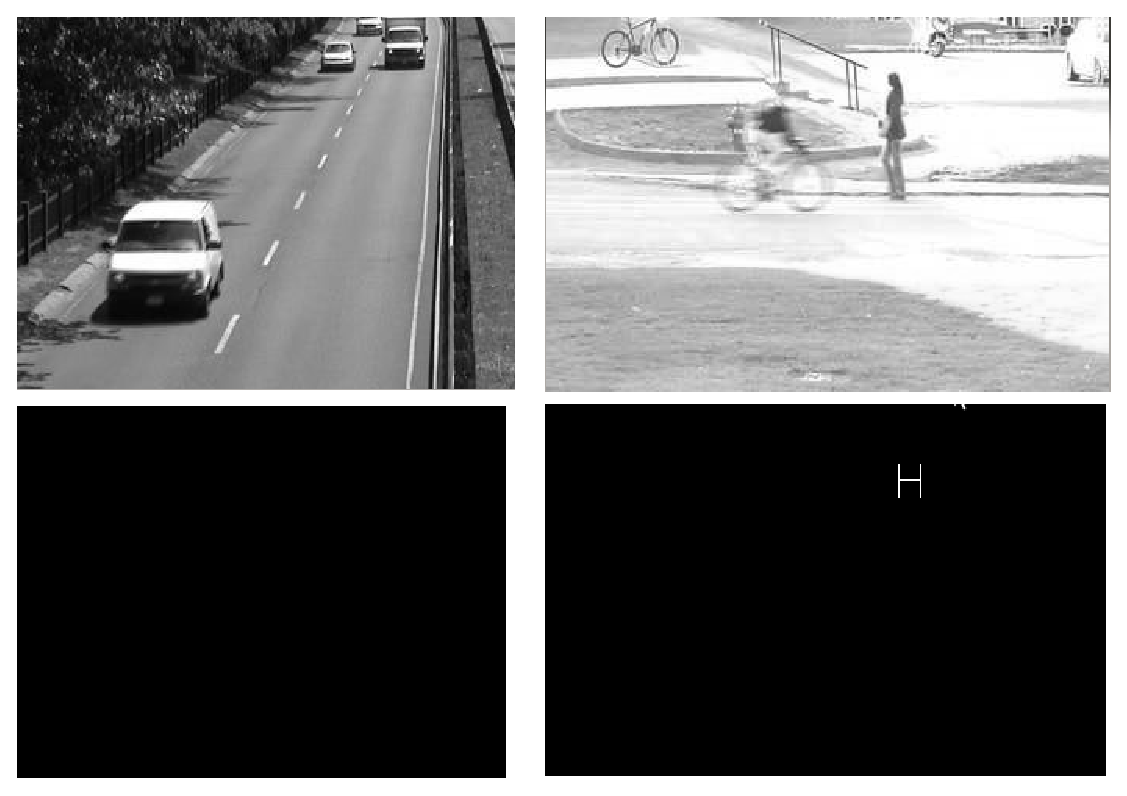
\includegraphics[height=300pt]{Figures/negative_inputs}
\caption{Input and output of pipeline in case of negative images}
\label{negative_inputs}
\end{figure}

\indent We have implemented and executed SKELMOT, Haar-like~\cite{19} and
covariance~\cite{19} feature based detection algorithm on both x86
desktop computer and embedded ARM platform. Comparison of execution time
has been shown in Fig.\ref{pipeline_execution_time}. It shows a
definite improvement in execution speed of SKELMOT over HAAR and covariance
feature based approach.  SKELMOT takes just 3.6 ms on the average, while
HAAR and covariance feature based algorithm take around 20 ms and 248 ms
respectively per frame on x86 platform having DMIPS = 800. Comparison of
timing on ARM platform with DMIPS = 44 shows that SKELMOT takes 182 ms
on the average, while HAAR and covariance feature based algorithm take
around 942 ms and 4.65 s respectively per frame.

\begin{figure}[!t]
\centering
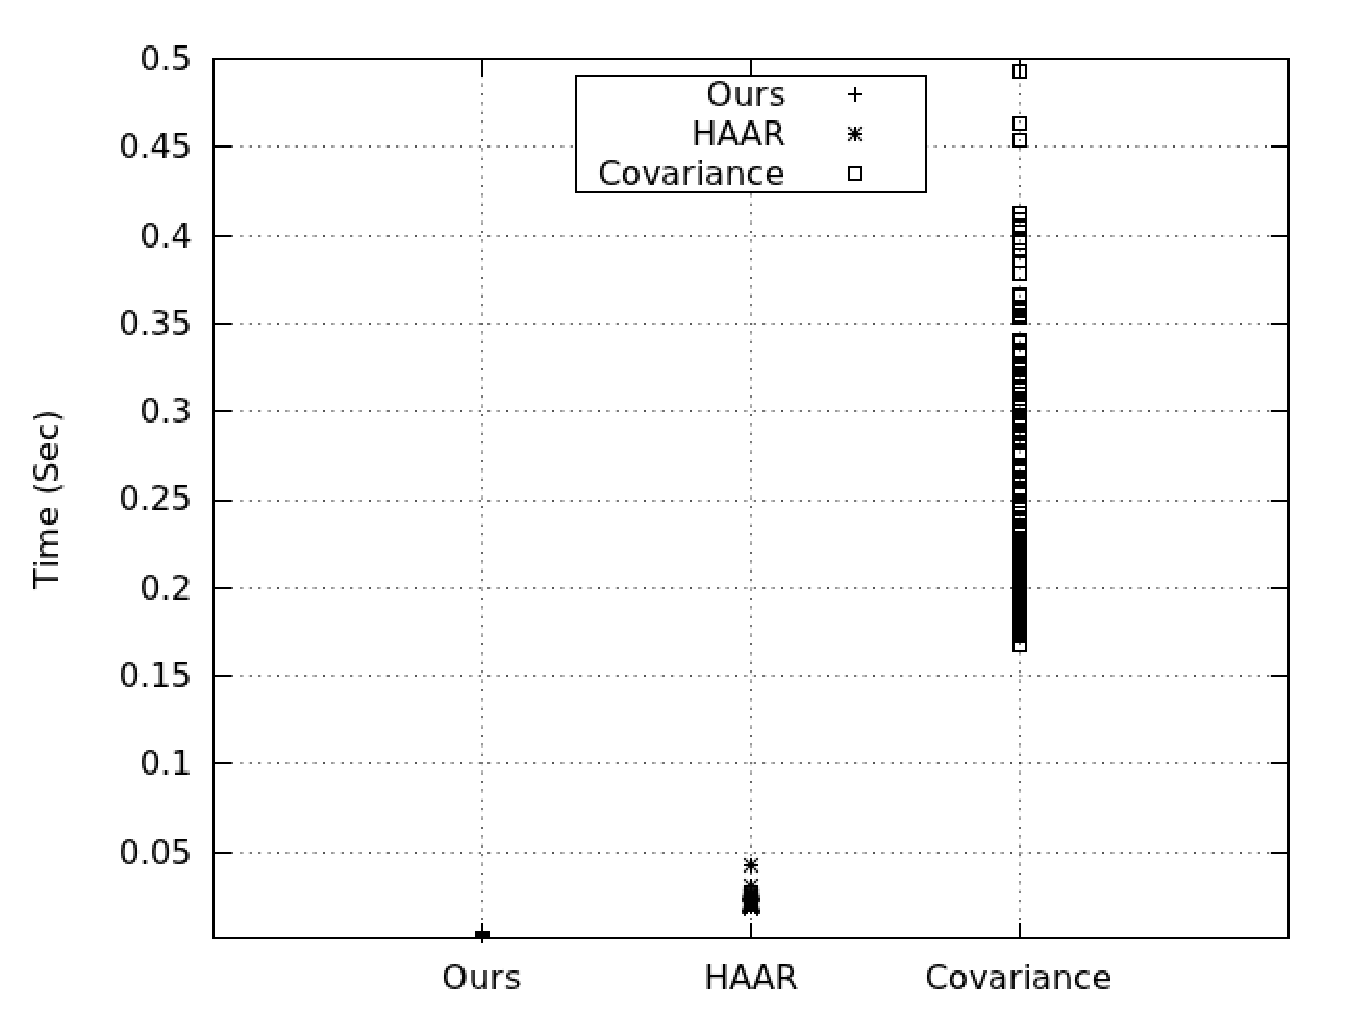
\includegraphics[scale=0.30]{Figures/pipeline_execution_time}
\caption{Execution time of evaluated algorithms on ARM and x86
platform}
\label{pipeline_execution_time}
\end{figure}
\section{Conclusion}
\indent We have seen that method based on covariance or Haar-like
descriptor is very slow in comparison with skeleton motion descriptor.
Therefore, if a surveillance application requires to identify moving
person, then we might not need to use complex algorithm to get real time
performance with low cost embedded platform. By using proposed
algorithm, we can save a lot of computational power. However, if we wish
to detect human from still frame, then we need to go for other methods.
To use other methods such as Haar or covariance features based
descriptor in real time environment, we recommend to implement them in
hardware. This dedicated hardware can further be used with low end
micro-controller to achieve end result.
\section{Future work}
Future work may be carried in following directions:
\begin{enumerate}
\item Test of this algorithm with real camera connected and Zigbee
network will provide good confidence to use it.
\item A research work may be initiated to see actual power saving using
such a low complexity pipeline.
\item There can be improvement in blob tracking algorithm to predict
next position on the basis of past N number of frames.
\item We have seen that low end micro-controller is not able to work with
single frame human detection algorithms. These algorithm can either run on
high performance CPU, or GPU. A work can be initiated to implement such
algorithms in hardware and then to use this hardware with low end
micro-controller. It would be interesting to see difference between power
consumption of two systems.
\end{enumerate}

 %future work

%% ----------------------------------------------------------------

\label{Bibliography}
\addtotoc{Bibliography}
\lhead{\emph{Bibliography}}  % Change the left side page header to "Bibliography"
\bibliographystyle{ieeetr}  % Use the "unsrtnat" BibTeX style for formatting the Bibliography
%\bibliographystyle{apalike}
\bibliography{Bibliography}  % The references (bibliography) information are stored in the file named "Bibliography.bib"
\cleardoublepage


\addtotoc{About the Author}
\lhead{\emph{About the Author}}
\huge\textbf{About the Author}

\begin{sloppypar}
\normalsize
Pratyush Anand was born in Darbhanga, India, in 1980. He graduated in
Electronics Engineering from N.I.T. Jamshedpur in 2003. He joined
Defence Research and Development Organization as Scientist 'B' in August
2003. He left this job in August 2005 and joined ST Microelectronics.
Currently he is working there as Engineering Specialist. He joined
Indian Institute of Technology Delhi as a part time MS(Research) student
in Computer Technology, Department of Electrical Engineering in 2010. He
has authored few Linux mainline drivers as well as contributed in
several other driver’s development around USB and PCIe. His research
interest include Embedded System, Low power system, High speed
interfaces, Surveillance system etc.
\end{sloppypar}


\end{document}  % The End
%% ----------------------------------------------------------------
